%%%%%%%%%%%%%%%%%%%%%%%%%%%%%%%%
\section{Detector monitoring and slow control}
\label{sec:detmonitoring}

The scope of the ProtoDUNE-SP detector control system (DCS) includes the design, procurement, fabrication, testing,
and delivery
of a comprehensive monitoring, control and safety system for the protoDUNE detector.

The responsibility for the system is split between ProtoDUNE-SP and CERN: 
\begin{itemize}
\item	The ProtoDUNE-SP collaboration is responsible for all devices that will be installed and cabled inside 
the cryostat, the sensors needed to monitor the cryostat and its content, and the specifications for the system. % needs. 
\item	CERN is responsible for the implementation of the control system elements outside the cryostat (hardware, firmware and software), including the high-voltage and low-voltage power supplies necessary for the detector operation.
\end{itemize}

This section describes %the monitoring devices and sensors inside the cryostat, 
the main requirements, 
constraints and assumptions of the control system, and its general structure and components. 

%%%%%%%%%%%%%%%%
\subsection{Monitoring devices and sensors}
\label{sec:mon-dev-sensors}

The protoDUNE-SP apparatus includes instrumentation beyond the TPC and the photon detectors to ensure that the condition of the liquid argon is adequate for operation of the TPC. This instrumentation includes gas analyzers to monitor the purge of the cryostat and ensure that any remaining atmospheric contamination is sufficiently low, thermometry to monitor the cryostat cool-down and filling, purity monitors to provide a rapid assessment of the electron drift-lifetime independent of the TPCs, and a system of internal cameras to help locate any sparks due to high voltage breakdown in the cryostat.

In addition, sets of precision temperature sensors are being deployed to measure the temperature gradients inside the protoDUNE cryostat. These temperature measurements exploit the opportunity protoDUNE-SP provides to check the predictions of the Computational Fluid Dynamics models being used to design the argon flow in the (much larger) DUNE cryostat.

The CERN Neutrino platform is providing the essential measurements of the cryostat pressure and external environmental conditions.

%here you are ...
The instrumentation is designed to establish the quality and stability of the detector environment and to help diagnose the source of any changes in the detector operations. In addition, an extensive set of temperature measurements is planned in order to provide input for the validation of the fluid dynamic models to be used in simulations of the full DUNE apparatus.


%%%%%%%%%
\subsubsection{Purity monitors} 
Three purity monitors (PrM) with sensitivity
%modification  in the ppt range 
to electron drift lifetimes from $\sim$100~microseconds up to a few milliseconds
%end
will be used to provide a rapid and direct determination of the 
% impurity content 
electron drift lifetime
of the LAr inside the ProtoDUNE-SP cryostat. These PrMs have been generously provided by ICARUS~\cite{Amerio:2004ze} 
after being decommissioned from the T600. 
The design has been replicated with small modifications
for MicroBooNE and 
a number of  R\&D test experiments at Fermilab. Inside the ProtoDUNE-SP the monitors are arranged in a vertical 
column
located behind the APA planes on the Jura side (see Figure~\ref{fig:cryo-side-names}). 
Two of the monitors are supported from the large flange on the manhole, while one is attached directly to the floor of the cryostat.
Ports
 with ConFlat seals on the blanking flange will be made available for
 HV/Signal/Optical Fiber feedthroughs.
 One monitor will be at the height of the top of the APA,
 one at mid-height, and one at the very bottom near the LAr-return manifold, %for the return LAr distribution 
which will allow it to monitor
the purity of the LAr entering the cryostat after the purification process.  

\begin{cdrfigure}[A purity monitor from ICARUS T600 ]{IcaPrM}{Picture of a purity monitor from the ICARUS T600, now available for installation in the ProtoDUNE-SP detector
%modification addition
. The photocathode is at the left, the drift region is defined by the ring-shaped electrodes, and the anode is at the right.}
%end 
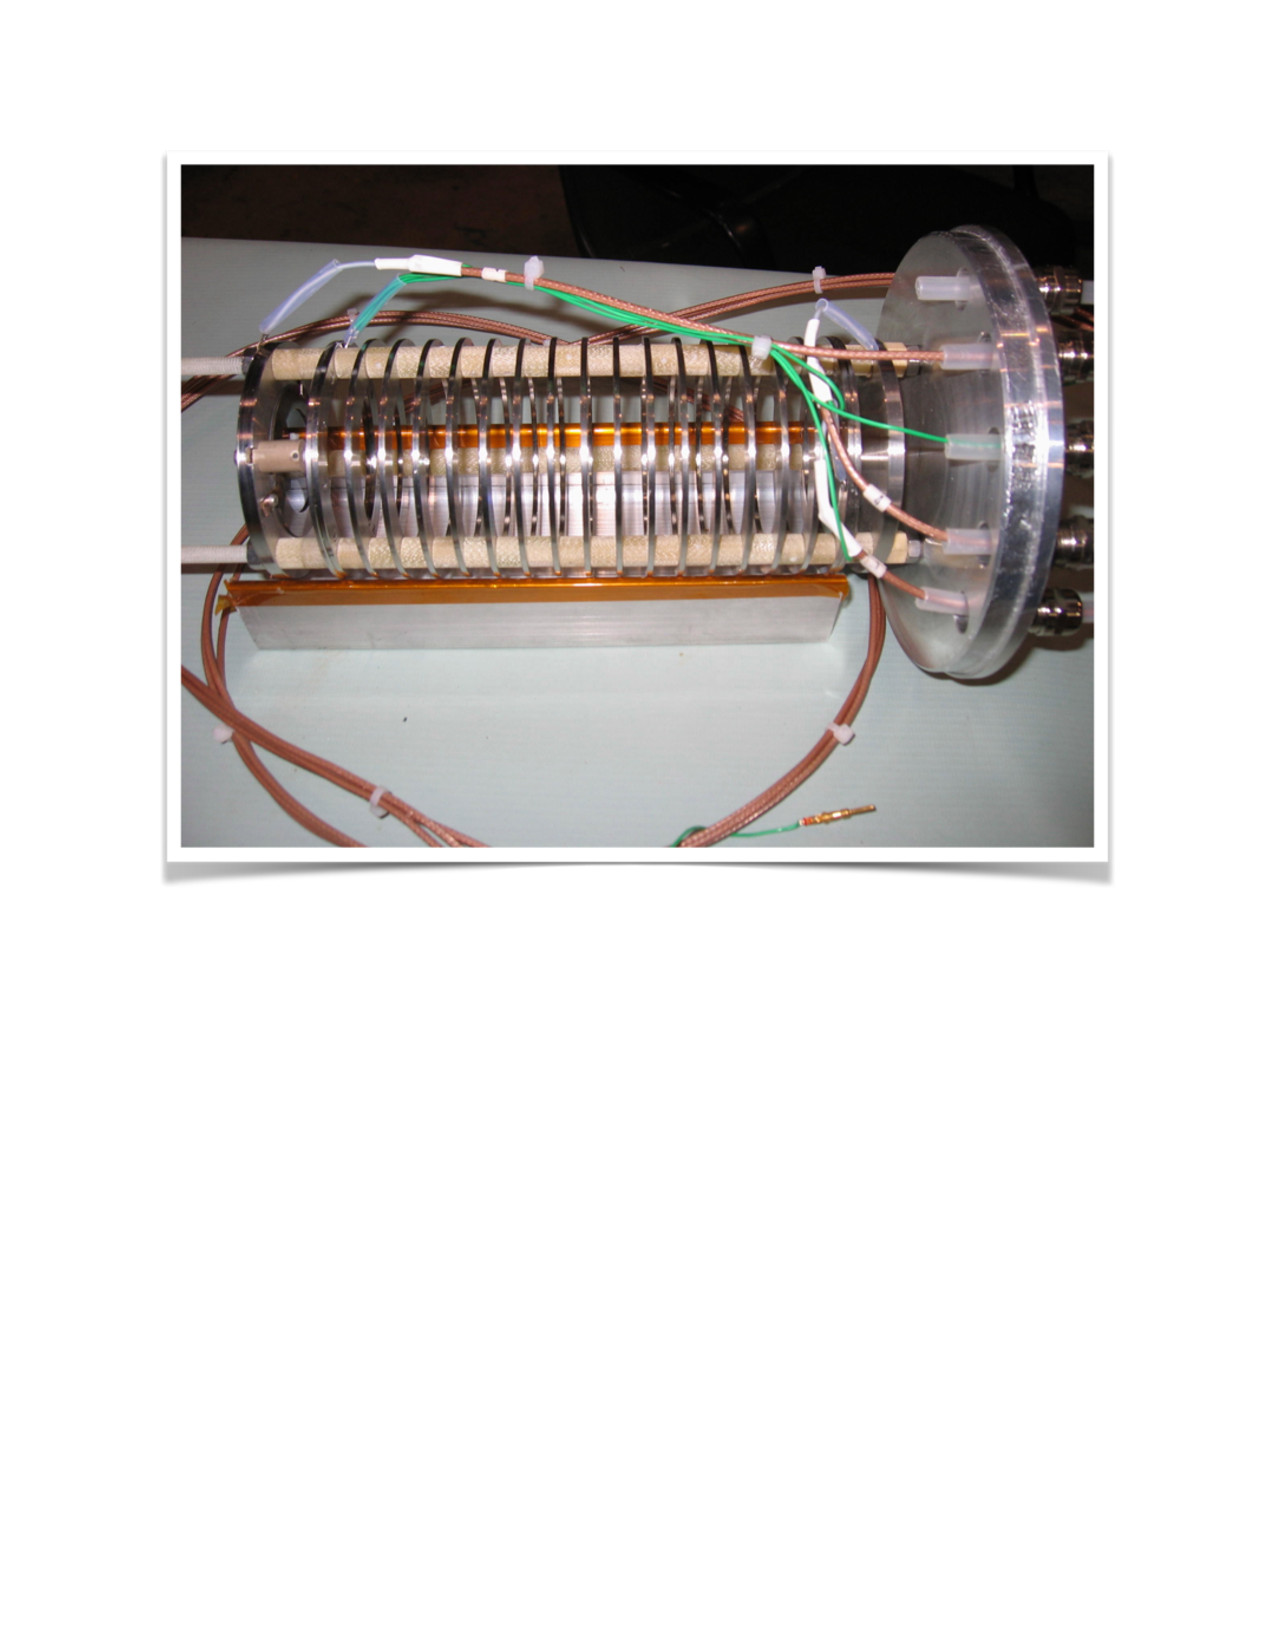
\includegraphics[width=0.5\textwidth]{IcaPrM.pdf} 
\end{cdrfigure}

The three PrMs, one of which is pictured in Figure~\ref{fig:IcaPrM}, are currently being refurbished with new gold photocathodes and new quartz fibers. The drift length  (25~cm) is the same for all them. 
%modification removal Using parts of another (available) PrM to extend the drift length of one of the three (e.g., to 40~cm) for more precise measurements of the longer $e-$ lifetimes is currently under consideration. %considered as an open option.
%end
The mechanical  design of the string and the connection to the manhole flange at the top 
% modification removal `end, and the fastening of the string at the bottom '
%modification replacement structure
%end
%are subject of a detailed ongoing engineering study. 
are under development.

A single PrM will be installed at the output of the purification filter system using a port that is available for this purpose. This installation will require DUNE to provide not only the purity monitor system but the vessel that will contain the PrM and the argon it is sampling.

%modification removal An additional PrM at the bottom on the opposite side of the cryostat would be useful for %comparing 
%with the response from the other PrM at the same height and thus 
%checking %the uniformity of 
% monitoring variations in the quality of 
%the LAr at that level, and providing information for the fluid-dynamics computation inside the cryostat. \\
%end

%modification addtion
%%%%%%%%%
\subsubsection{Analytic gas equipment}

A system of gas analyzers will be used to certify the deliveries of argon, to monitor the effectiveness of the purging of the cryostat, and to monitor the state of the argon under operation. Commercial devices with 1 part per billion (ppb) and better sensitivity to oxygen and water, and with 100-ppb sensitivity to nitrogen are available and appropriate. A valve switch-yard is provided to allow the analyzers to sample either the liquid or the ullage in the cryostat, and to sample other points of interest in the argon system.


%%%%%%%%%
\subsubsection{Vertical temperature gradient monitor}

	%SP
	Precise %SPmonitoring 
	measurements of the temperature, specifically of the temperature gradient, %SPgradient 
	as a function of LAr depth are %considered highly important as 
	an important input for fluid dynamics modeling and simulations.  The ProtoDUNE cryostats are the largest argon cryostats ever constructed for a LArTPC and present the best opportunity to validate the models used in the design and simulation of the full DUNE detector modules. The installation of two sets of devices with high-precision temperature measurements
	%the precise measurement of the LAr temperature across 
	along almost the entire height of the LAr volume %inside the cryostat 
	has been included in the internal instrumentation plan for this purpose. The two sets allow testing both the transverse and vertical components of the models and provide an opportunity to test different measurement technologies on a relevant scale. 
%	A precision better than 50~mK in the temperature measurement is assumed as target requirement for the device. 
	Commercial calibrated resistance temperature detectors (RTDs) with 15-mK precision at LAr temperature are well suited to this application, recognizing that the temperature probe wiring and signal transport outside the cryostat require considerable care in order to maintain % is necessary to prevent spoiling 
	the intrinsic precision of the probe.
	
One of  %current base option  
the vertical profile monitors is supported from a port located behind the APA plane. It consists of a series of RTDs positioned at $\sim$30 to 50~cm intervals %distance between one another 
along a rigid structure. %the flange %on one of 
 %on the top side 
%at the top of the cryostat. 
A special multi-pin FT is mounted on the flange %is necessary 
for the signal extraction and readout from a temperature controller.  Cross calibration of the RTDs in place is to be achieved by stepping the structure so that two adjacent RTDs can sample the temperature in the same location.
The mechanical design, including the cable routing up to the multi-pin FT, is under study.
%Also in this case, the engineering study of the mechanical structure has to be developed in detail, including cables routing up to the multi-pin FT. \\
The second profile monitor uses a port located on the downstream end of the cryostat. Studies of cross calibration of the RTDs are under way. 

A number of RTDs will also be positioned at different heights %on the APAs and 
on the cryostat walls to monitor the temperature %drop 
during the %cooling 
cooldown process. There will also be some RTDs on the cryostat roof,  RTDs on the argon inlet and outlet lines, and, just for luck, an RTD on each of the purity monitors.
%phase.

%%%%%%%%%
\subsubsection{Webcams inside the cryostat}
	Based on %the solution 
	a system developed by ETH Zurich for WA105, six commercial webcams, sealed inside a specially developed metal case with a ConFlat optical window to allow operation at cryogenic temperatures, are located inside the cryostat. They are positioned at strategic points to allow inspection of the interior during filling and commissioning, % operations, 
	and the detection and recording of possible sparks in locations of high %the highest 
	electric field intensity, such as the HV feedthrough. A system of these cameras has been installed in the 35t field cage test at Fermilab and the lessons learned will be incorporated in the final design.
	
%%%%%%%%%
\subsubsection{Level meters and pressure sensors.}
	Level Meters and pressure sensors are important for both cryogenics and detector operation. CERN is providing the devices for these measurements, a level meter based on a differential pressure gauge and a redundant pair of sensors to measure the pressure in the ullage. CERN will also provide a weather station to give measurements of the local temperature and atmospheric pressure.


%%%%%%%%%%%%%%%%%%%%%%%%%%%%%%%%%%%%%%%%%%%%%%
\subsection{Slow control system}
\label{sec:slowcontrol}

The design of the ProtoDUNE-SP safety and control system is largely based on the experience gained in collaboration with ETH Zurich during the pilot WA105 project at CERN. The components of this system and their functions are as follows:
\begin{itemize}
\item	The Process Control System (PCS) reads temperature sensors including the Vertical T Gradient monitors, 
the pressure sensors in the gas ullage, the liquid argon level meter,
the purity monitors inside the cryostat, and the trace analyzers (O$_2$, N$_2$, H$_2$O) in the external recirculation line.
\item	The Detector Control System (DCS) monitors and controls the low-voltage (LV) and high-voltage (HV) from the power supplies.
\item	The Detector Safety System (DSS) performs temperature surveys and monitors interlocks and alarms.
\end{itemize}

The supervisory software is based on the JCOP framework, an integrated set of software tools originally developed for the control of the LHC experiments and 
now used in several more experiments at CERN. The framework provides a graphical user interface to visualize the trends of monitored values and 
alarm/interlock conditions. These values and alarms are automatically stored in a dedicated database for offline use. Remote monitoring is possible via a web 
interface.

The responsibility for the system is split between ProtoDUNE-SP and CERN: 
\begin{itemize}
\item The ProtoDUNE-SP experiment is responsible for all sensors, power distribution, etc., inside the cryostat, 
as well as for defining the system specifications, I/O parameters and control, and safety logic. \fixme{In general I don't like to use ``etc'' because it's unclear what else is included. Anne}
\item CERN EP/DT-DI  is responsible for developing and testing the supervisory control of the system and data acquisition (SCADA).
This includes connecting the control system to the cryogenics instrumentation inside the cryostat and to all the systems that require monitoring and/or control, such as power supplies, cameras and lighting. 
\end{itemize}

In particular, CERN EP/DT-DI is developing a dedicated readout system based on National Instrument modules to allow the 
multiplexing of the RTDs inside the cryostat.  A prototype of this readout system is currently under test.
 
Figure~\ref{fig:dcsdesign} shows the general architecture of the control and safety system for ProtoDUNE-SP, including the PCS, the DCS and the DSS.

\begin{cdrfigure}[Process control, detector control and safety systems]{dcsdesign}{Proposed architecture and technical solution of the detector control and safety system.}
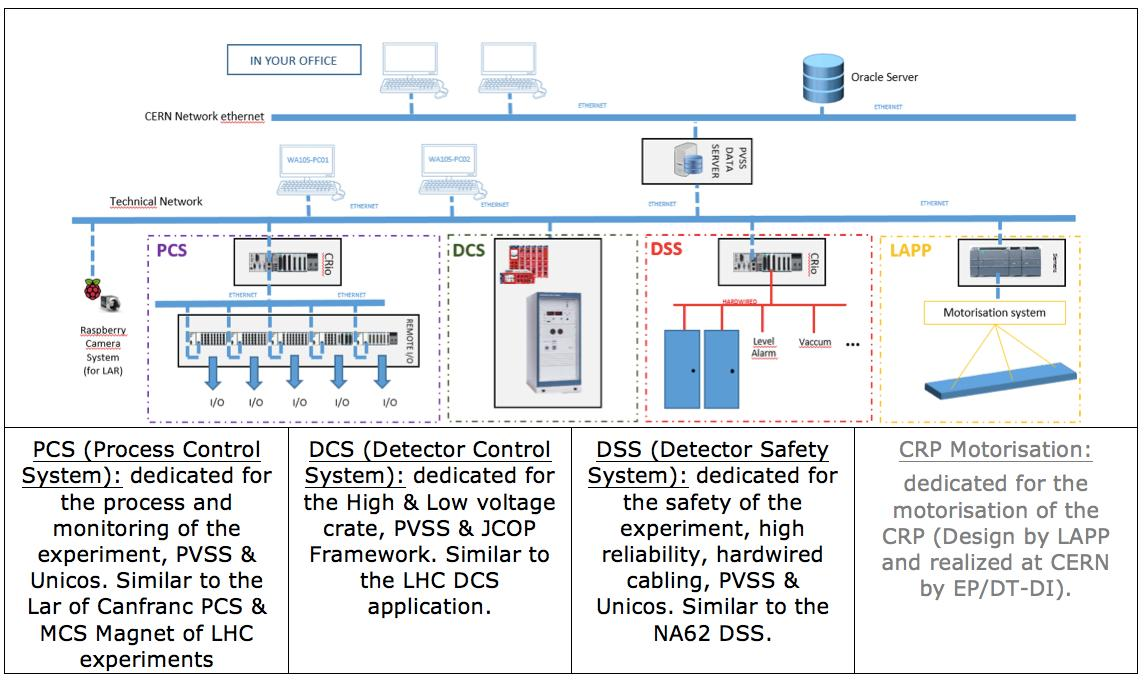
\includegraphics[angle=90, height=0.9\textheight]{DCS_Design}
\end{cdrfigure}

The control system is composed of:
\begin{itemize}
\item a chassis for electrical distribution (380~Vac, 220~Vac, 24~Vdc redundant);
\item two chassis for the PCS, composed of an FPGA, signal conditioners, interface, and cabling;
\item one chassis for the DCS,  composed of an interface for LV/HV monitoring \& control; 
\item a chassis for the DSS, composed of an FPGA and relays for the safety of the experiment; 
\item a chassis for a PC data acquisition \& supervision (PVSS SCADA Supervisor), composed of a computer with a display monitor, a switch and a server; 
\item four chassis for the remote I/O to capture signals close to the detector and to avoid multi-cabling structure; and
\item one chassis for the HV, controlled by the slow-control system. 
\end{itemize}
All these elements will be mounted in 19-in. racks.


